\chapter{Boundary Conditions}
\label{chapter:boundary-conditions}

In an LBM simulation, enforcing boundary conditions involves determining unknown incoming distributions at boundary nodes based on known outgoing distributions and other auxiliary information.
Depending on how the boundary is encoded into the lattice, LBM simulators distinguish between
\begin{itemize}
    \item \textbf{Wet-Nodes} The boundary conditions are applied directly on the fluid nodes at the boundary. This is usually done after streaming.
    \item \textbf{Link-Wise} The boundary conditions are applied between fluid nodes and solid nodes. This is usually done during streaming.
\end{itemize} \cite{olbug:18}.

\section{Linear Boundary Formulation}
\label{sec:bc-formulation}

Due to the linear constraints of quantum operations, I focused on modeling the unknown distributions as linear combinations of the known distributions at the boundary nodes.
This is a well known wet-node approach, detailed by \cite{zou1997pressure}.
Additionally, due to the norm-preserving nature of quantum operations, I restrict myself to boundary conditions that preserve the total density at the boundary node.
Mathematically, this can be expressed as:

\begin{equation}
f_i^{in} = \sum_j B_{ij} f_j^{out}
\end{equation}

Or in matrix form:
\begin{equation}
\mathbf{f}^{in} = B \cdot \mathbf{f}^{out}
\end{equation}

\section{Quantum Implementation via LCU and SVD}
\label{sec:bc-implementation}

Since the boundary matrix $B$ is generally non-unitary, it cannot be directly implemented as a quantum gate.
To address this, I employ the Linear Combination of Unitaries (LCU) technique \cite{childs2012hamiltonian}.
This is already used in many QLBM implementations to handle the collision step \cite{budinski2021quantum}.
Because the collision operator is diagonal, it was straightforward to express it as a linear combination of two unitaries:
\begin{equation}
C = \frac{1}{2} (C + i\sqrt{I - C^2}) + \frac{1}{2}(C - i\sqrt{I - C^2})
\end{equation}

The Boundary operator $B$ is unfortunately not diagonal.
For simplicity, I opted to decompose it using Singular Value Decomposition (SVD):
\begin{equation}
    B = U \Sigma V^{\dagger}
\end{equation}
where $U, V$ are unitary and $\Sigma$ is diagonal. Using this fact, $\Sigma$ can be decomposed as a linear combination of two unitaries, and $U$ and $V^{\dagger}$ distributed to obtain a linear combination for $B$:
\begin{equation}
    B = \frac{1}{2} (U (\Sigma + i\sqrt{I - \Sigma^2}) V^{\dagger} + U (\Sigma - i\sqrt{I - \Sigma^2}) V^{\dagger})
\end{equation}
This allows implementing $B$ using one ancilla qubit with a 50\% success probability.

\section{Circuit Optimization}
\label{sec:bc-optimization}

As discussed, LCU is already employed for the collision step, already resulting in a 50\% success probability per iteration.
If another LCU step is added for the boundary conditions, the overall success probability would drop to 25\%.

The idea here was to move the boundary conditions step before the streaming step, and combine the collision and boundary operators into a single matrix.
This is equivalent to considering the boundary conditions as a fundamental part of the collision process, instead of a separate step.
\begin{equation}
    C_{combined} =  B \cdot C
\end{equation}
I then perform SVD on this combined matrix $C_{combined}$. This maintains a single LCU step per iteration, preserving the 50\% success probability.

\todo{REVISION: improve the probability discussion with LCU optimization details}
\todo{REVISION: add section about post-to-pre streaming trick and discoveries}

This shift does involve adjusting the boundary condition matrix to account for the fact that unknown distributions are now streamed immediately after being computed.
While I have not proven that it is always possible to rewrite a post-streaming boundary condition as a pre-streaming one, I have managed to do so for the case I tested.

\section{Complexity Impact}
\label{sec:bc-complexity}

\todo{Write BC complexity analysis: impact of SVD decomposition, controlled unitaries, comparison with diagonal-only collision.}

\section{Experimental Validation}
\label{sec:bc-validation}

I validated the method using a 1D Advection-Diffusion setup.
This was chosen due to simplicity, but in theory nothing prevents the method from being applied to higher dimensions or more complex collision operators.
The simulation parameters were as follows:

\begin{itemize}
    \item \textbf{Lattice:} 1D grid, size 32.
    \item \textbf{Setup:} D1Q3 (Left, Rest, Right velocities).
    \item \textbf{Initial Condition:} Gaussian hill centered in the domain.
    \item \textbf{Velocity Field:} $u=0.1$ (rightward) for $t \in [0, 75]$, then $u=0$ for $t \in [75, 150]$.
    \item \textbf{Boundary Conditions:} Solid walls at both ends, populations that would stream into the boundary are instead redistributed to be stationary. Equations for right boundary:

    \[f_{-1}^{post} = f_{-1}^{pre} \]
    \[f_{0}^{post} = f_{0}^{pre} + 1.0 \cdot f_{1}^{pre}\]
    \[f_{1}^{post} = 0 \]
\end{itemize}

I performed both a classical simulation (implementing the same matrix logic) and the quantum simulation (statevector simulator).
The classical simulation visually matched the expected behavior of a solid wall.

\begin{figure}[H]
    \centering
    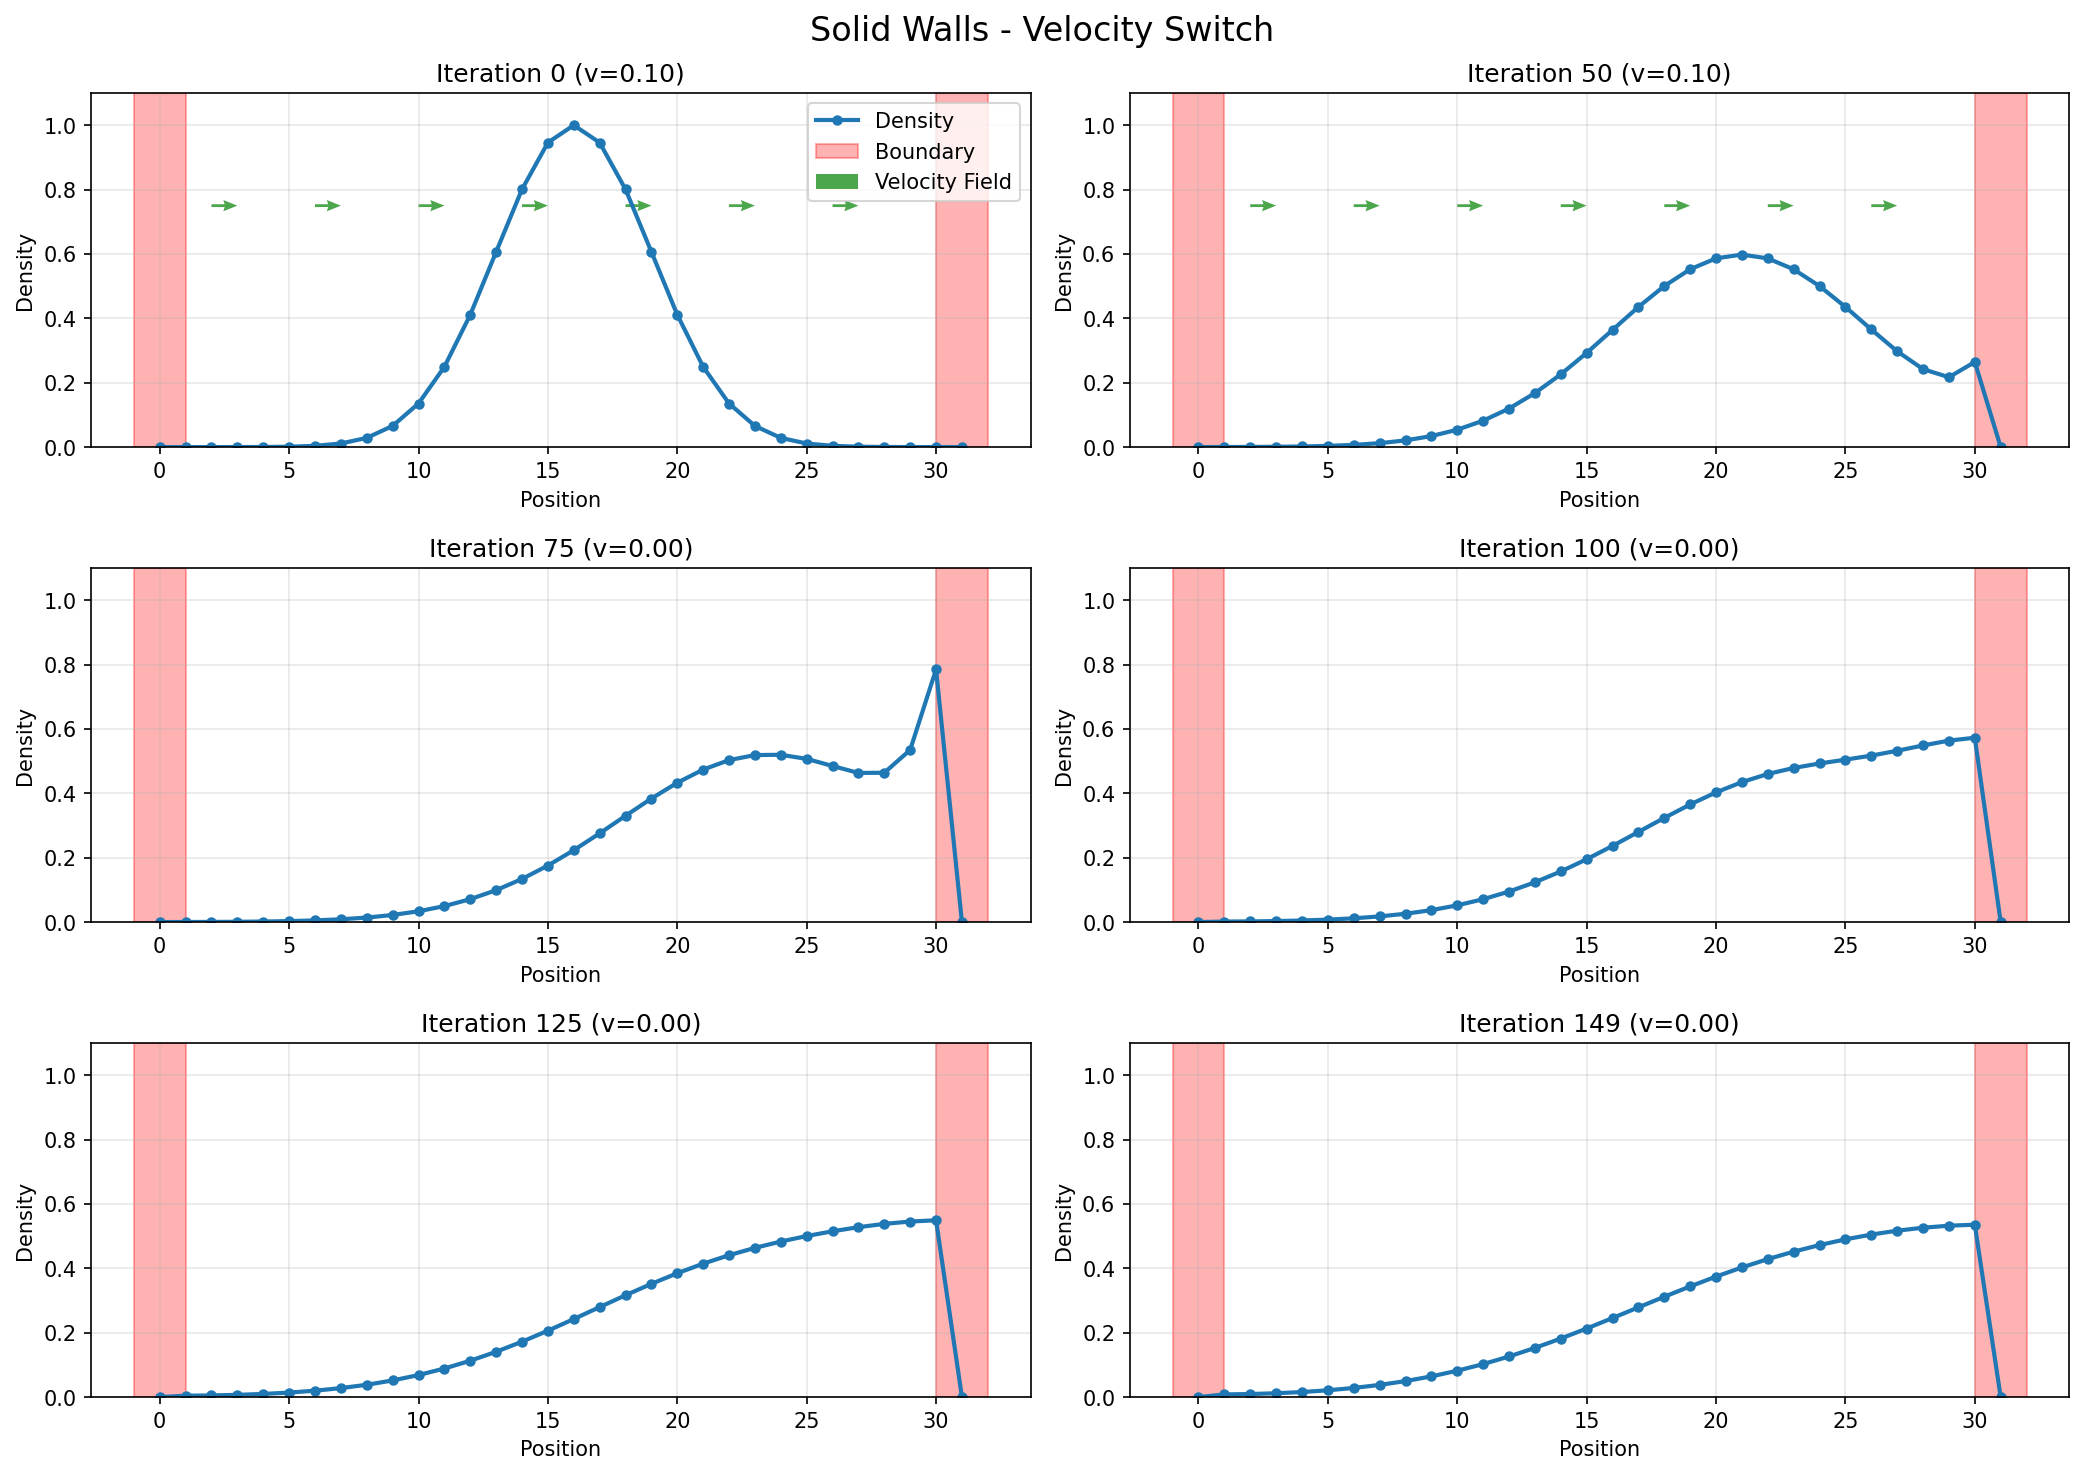
\includegraphics[width=0.8\textwidth]{src/img/figures/snapshots.png}
    \caption{Classical simulation results showing the Gaussian profile being contained by the solid walls. Given enough iterations, it would eventually flatten completely.}
    \label{fig:bc_snapshots}
\end{figure}

The quantum simulation was validated by computing the Root Mean Square Error (RMSE) between the classical and quantum results at each time step.

\begin{figure}[H]
    \centering
    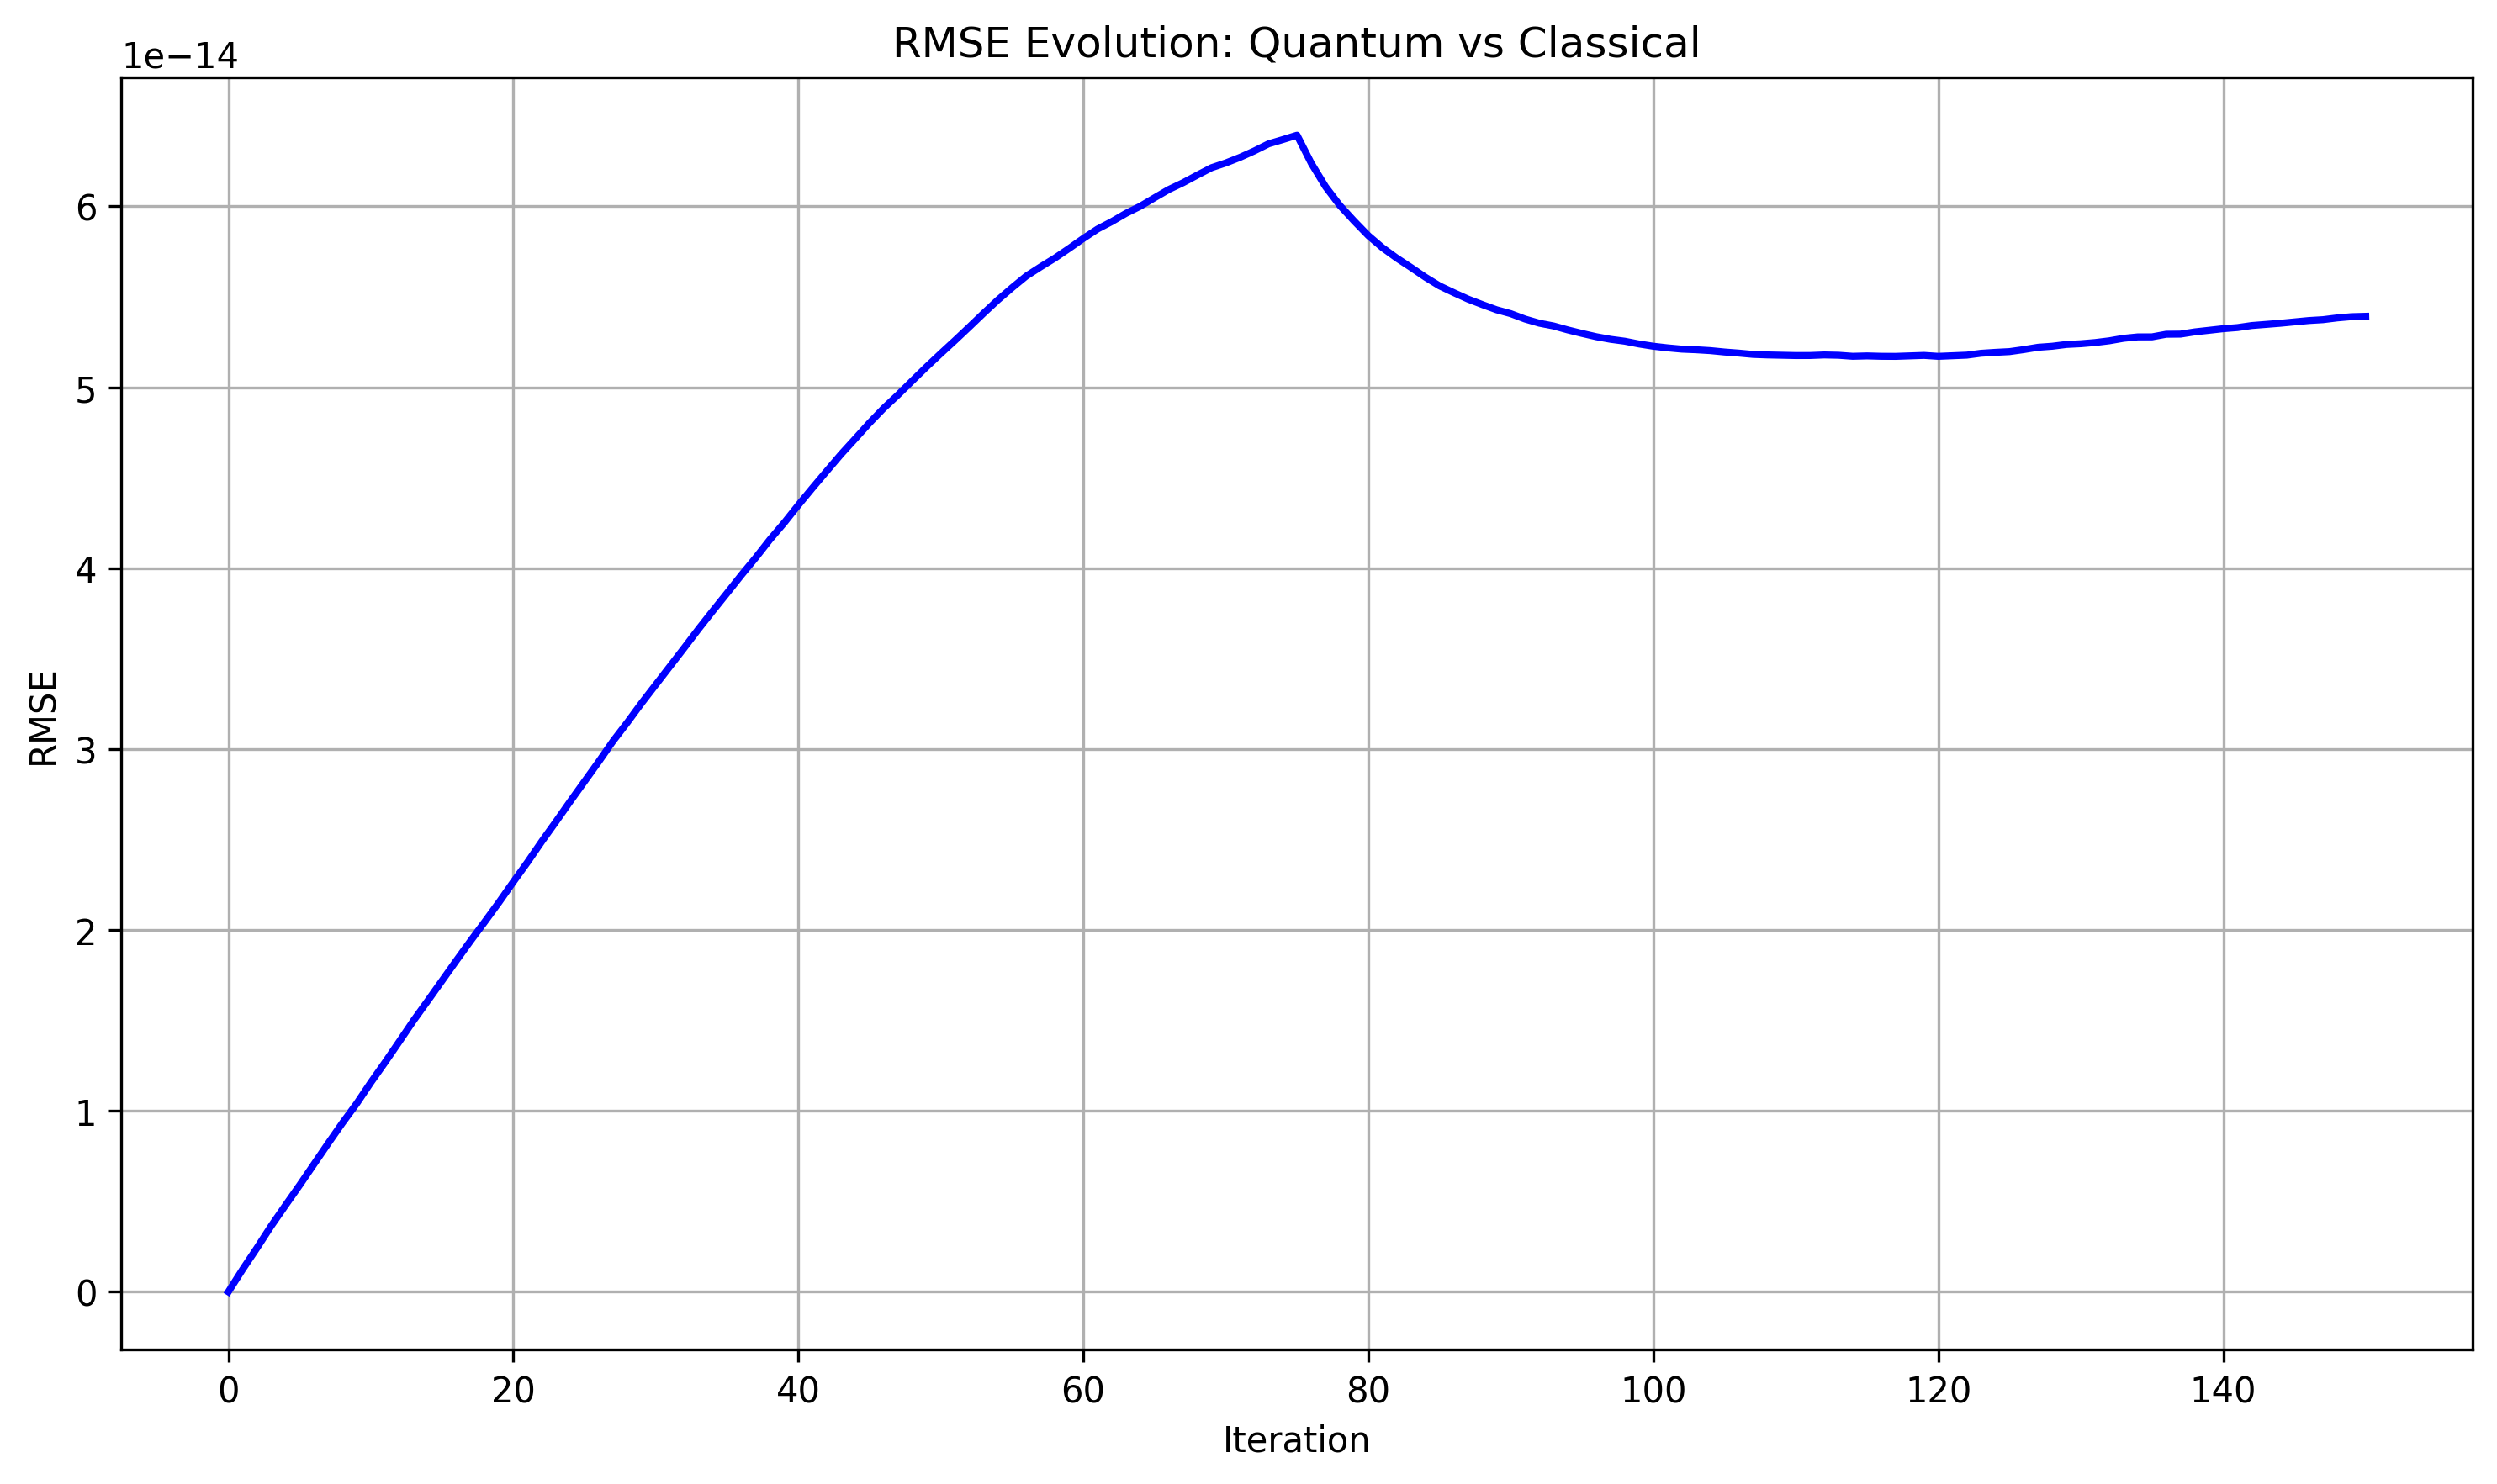
\includegraphics[width=0.8\textwidth]{src/img/figures/rmse_comparison.png}
    \caption{RMSE comparison between Classical and Quantum implementation demonstrating numerical precision agreement.}
    \label{fig:bc_rmse}
\end{figure}

\todo{REVISION: add 2D boundary condition experiments}
